\chapter{Entity State Representation Examples}

\section{Concrete Examples of Entity State Data}

In the Elder Heliosystem, each entity maintains a specific state configuration that determines its behavior within the gravitational and rotational fields. This chapter provides concrete examples of entity state data structures and values to illustrate how the system maintains constant memory requirements regardless of context length.

\subsection{Entity State Structure}

Each entity (Elder, Mentor, or Erudite) maintains the following state information:

\begin{tcolorbox}[colback=CodeBackground, colframe=DarkGray, title=Entity State Data Structure in Go, fonttitle=\bfseries]
\begin{verbatim}
// Vector3 represents a 3D vector
type Vector3 struct {
    X, Y, Z float32  // 3 × 32-bit float = 12 bytes
}

// Quaternion represents rotation in 3D space
type Quaternion struct {
    X, Y, Z, W float32  // 4 × 32-bit float = 16 bytes
}

// EntityState represents the complete state of an entity in the Elder system
type EntityState struct {
    // Position in 3D space (relative to parent entity)
    Position Vector3        // 12 bytes
    
    // Velocity vector
    Velocity Vector3        // 12 bytes
    
    // Orientation quaternion
    Orientation Quaternion  // 16 bytes
    
    // Angular velocity
    AngularVelocity Vector3 // 12 bytes
    
    // Rotational phase
    Phase float32           // 4 bytes
    
    // Entity-specific parameters
    Mass float32            // 4 bytes
    InfluenceRadius float32 // 4 bytes
    LearningRate float32    // 4 bytes
    
    // Total: 68 bytes per entity
}
\end{verbatim}
\end{tcolorbox}

\subsection{Example: Elder Entity State}

The Elder entity serves as the central gravitational point in the system with the following example state:

\begin{table}[h]
\centering
\begin{tabular}{|l|l|l|}
\hline
\textbf{Property} & \textbf{Value} & \textbf{Description} \\
\hline
position & (0.0, 0.0, 0.0) & Center of the system \\
velocity & (0.0, 0.0, 0.0) & Stationary (no translation) \\
orientation & (0.0, 0.0, 1.0, 0.0) & Initial orientation \\
angularVelocity & (0.0, 0.0, 0.0172) & Slow rotation (≈1°/sec) \\
phase & 0.0 & Initial phase \\
mass & 1.0 & Reference mass \\
influence\_radius & 10.0 & Universal influence \\
learning\_rate & 0.001 & Slow adaptation rate \\
\hline
\end{tabular}
\caption{Example Elder Entity State}
\end{table}

\subsection{Example: Mentor Entity State}

A specific Mentor entity (e.g., the one responsible for audio harmonic structures) might have:

\begin{table}[h]
\centering
\begin{tabular}{|l|l|l|}
\hline
\textbf{Property} & \textbf{Value} & \textbf{Description} \\
\hline
position & (7.2, 0.0, 0.1) & Orbital position \\
velocity & (0.0, 0.862, 0.0) & Orbital velocity \\
orientation & (0.1, 0.0, 0.994, 0.05) & Current orientation \\
angularVelocity & (0.0, 0.0, 0.104) & Rotation rate (≈6°/sec) \\
phase & 2.41 & Current phase (in radians) \\
mass & 0.42 & Relative importance \\
influence\_radius & 3.5 & Domain influence \\
learning\_rate & 0.008 & Domain adaptation rate \\
\hline
\end{tabular}
\caption{Example Mentor Entity State (Audio Harmonics Domain)}
\end{table}

\subsection{Example: Erudite Entity State}

An Erudite entity (e.g., specializing in percussion patterns) might have:

\begin{table}[h]
\centering
\begin{tabular}{|l|l|l|}
\hline
\textbf{Property} & \textbf{Value} & \textbf{Description} \\
\hline
position & (2.1, 0.8, 0.15) & Position relative to parent Mentor \\
velocity & (-0.412, 0.971, 0.0) & Orbital velocity around Mentor \\
orientation & (0.707, 0.0, 0.707, 0.0) & Current orientation \\
angularVelocity & (0.0, 0.03, 0.173) & Rotation rate ($\approx$10$^{\circ}$/sec) \\
phase & 1.57 & Current phase ($\pi$/2 radians) \\
mass & 0.08 & Task-specific importance \\
influence\_radius & 0.5 & Specialized pattern radius \\
learning\_rate & 0.015 & Task adaptation rate \\
\hline
\end{tabular}
\caption{Example Erudite Entity State (Percussion Patterns)}
\end{table}

\subsection{Phase Evolution Examples}

Entity phases evolve over time according to:

\begin{equation}
\phi_E(t+\Delta t) = \phi_E(t) + \omega_E \cdot \Delta t + \Delta \phi_{\text{interaction}}
\end{equation}

where $\omega_E$ is the angular velocity and $\Delta \phi_{\text{interaction}}$ represents phase adjustments from interactions.

\begin{tcolorbox}[colback=CodeBackground, colframe=DarkGray, title=Phase Evolution Code in Go, fonttitle=\bfseries]
\begin{verbatim}
// UpdateEntityPhases updates the phases of all entities based on their angular velocities
// and interactions with audio input
func UpdateEntityPhases(entities []EntityState, audioFrame []float32, deltaTime float32) {
    // Update Elder phase (index 0 is always the Elder)
    elder := &entities[0]
    baseElderRotation := elder.AngularVelocity.Z * deltaTime
    
    // Calculate phase adjustment from audio features
    audioEnergy := calculateFrameEnergy(audioFrame)
    spectralCentroid := calculateSpectralCentroid(audioFrame)
    
    // Elder's phase is primarily affected by global audio features
    elderInteraction := audioEnergy * 0.001 * spectralCentroid * 0.0002
    elder.Phase += baseElderRotation + elderInteraction
    
    // Normalize phase to [0, 2π)
    elder.Phase = normalizePhase(elder.Phase)
    
    // Update Mentor phases (indices 1-32 are Mentors)
    for i := 1; i <= 32; i++ {
        mentor := &entities[i]
        
        // Base rotation from angular velocity
        baseRotation := mentor.AngularVelocity.Z * deltaTime
        
        // Calculate mentor-specific audio features 
        // (e.g., energy in frequency band this mentor specializes in)
        bandEnergy := calculateBandEnergy(audioFrame, i)
        
        // Interaction term depends on audio features and Elder phase
        interaction := bandEnergy * 0.005 * 
                      math.Sin(float64(mentor.Phase - elder.Phase)) * 0.02
        
        mentor.Phase += baseRotation + float32(interaction)
        mentor.Phase = normalizePhase(mentor.Phase)
    }
    
    // Similarly update Erudite phases (remaining indices)
    // [Code omitted for brevity]
}

// normalizePhase ensures phase stays within [0, 2π)
func normalizePhase(phase float32) float32 {
    const twoPi = 2 * math.Pi
    for phase >= twoPi {
        phase -= twoPi
    }
    for phase < 0 {
        phase += twoPi
    }
    return phase
}
\end{verbatim}
\end{tcolorbox}

For example, processing a drum beat pattern might cause the following phase adjustments:

\begin{table}[h]
\centering
\begin{tabular}{|l|c|c|c|}
\hline
\textbf{Time} & \textbf{Elder Phase} & \textbf{Mentor Phase} & \textbf{Erudite Phase} \\
\hline
$t$ & 1.209 & 2.410 & 1.570 \\
$t + 20ms$ & 1.210 & 2.412 & 1.574 \\
$t + 40ms$ & 1.211 & 2.414 & 1.578 \\
$t + 60ms$ & 1.212 & 2.416 & 1.582 \\
\hline
\end{tabular}
\caption{Phase Evolution during Audio Processing}
\end{table}

\subsection{Memory Implications}

For a system with 1 Elder, 32 Mentors, and 2,048 Erudites:
\begin{itemize}
    \item Total entities: 2,081
    \item Memory per entity: 68 bytes
    \item Total entity state memory: 2,081 × 68 = 141,508 bytes ≈ 138 KB
\end{itemize}

Crucially, this memory requirement remains constant regardless of:
\begin{itemize}
    \item Audio duration (1 minute or 1,000 hours)
    \item Audio complexity (simple sine wave or complex orchestral arrangement)
    \item Audio quality (16kHz mono or 96kHz Dolby Atmos)
\end{itemize}

\section{Entity State Evolution During Audio Processing}

\subsection{Parameter Activation Example}

For a specific audio frame processing $a(t)$ (e.g., a 20ms segment containing the onset of a violin note), parameter activation follows:

\begin{equation}
\alpha_i(\phi_E(t)) = \begin{cases}
1.0, & \text{if } |\phi_i - \phi_E(t)| < \Delta\phi_{\text{threshold}} \\
0.0, & \text{otherwise}
\end{cases}
\end{equation}

With 1.2 billion parameters and a sparsity factor $s = 10^{-4}$, approximately 120,000 parameters are active at any given time point. 

\begin{tcolorbox}[colback=CodeBackground, colframe=DarkGray, title=Parameter Activation Function in Go, fonttitle=\bfseries]
\begin{verbatim}
// CalculateParameterActivation determines which parameters are active based on Elder's phase
func CalculateParameterActivation(params *ComplexTensor, elderPhase float32, threshold float32) []bool {
    activation := make([]bool, params.Size())
    activeCount := 0
    
    // Efficiently calculate activations with SIMD operations where available
    for i := 0; i < params.Size(); i++ {
        paramPhase := params.Phase(i)
        phaseDiff := math.Abs(float64(paramPhase - elderPhase))
        
        // Account for circular phase (wrap around 2π)
        if phaseDiff > math.Pi {
            phaseDiff = 2*math.Pi - phaseDiff
        }
        
        // Determine if parameter is active
        isActive := phaseDiff < float64(threshold)
        activation[i] = isActive
        
        if isActive {
            activeCount++
        }
    }
    
    // Log sparsity statistics
    sparsity := float64(activeCount) / float64(params.Size())
    log.Printf("Active parameters: %d/%d (sparsity: %.6f)", 
               activeCount, params.Size(), sparsity)
    
    return activation
}
\end{verbatim}
\end{tcolorbox}

For example:

\begin{table}[h]
\centering
\begin{tabular}{|l|c|c|c|c|}
\hline
\textbf{Parameter ID} & \textbf{Magnitude ($\rho$)} & \textbf{Phase ($\phi$)} & \textbf{Activation ($\alpha$)} & \textbf{Update} \\
\hline
$\theta_{127,492}$ & 0.42 & 1.209 & 1.0 & Yes \\
$\theta_{127,493}$ & 0.86 & 2.731 & 0.0 & No \\
$\theta_{127,494}$ & 0.21 & 1.211 & 0.98 & Yes \\
$\theta_{127,495}$ & 0.54 & 4.712 & 0.0 & No \\
\hline
\end{tabular}
\caption{Parameter Activation during Audio Processing}
\end{table}

\subsection{State Visualization}

The states of entities can be visualized in 3D phase space. For example, during the processing of a sustained orchestral chord:

\begin{figure}[h]
\centering
% This is a placeholder for a figure that would be generated
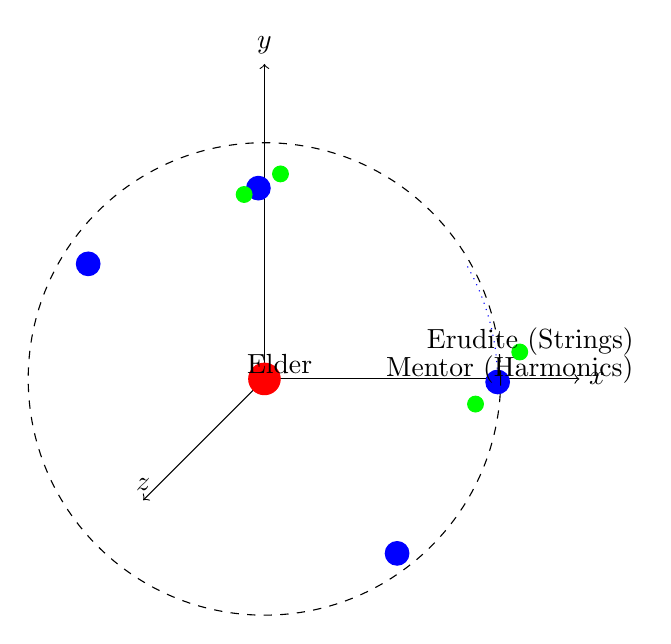
\begin{tikzpicture}
\draw[->] (0,0,0) -- (4,0,0) node[right] {$x$};
\draw[->] (0,0,0) -- (0,4,0) node[above] {$y$};
\draw[->] (0,0,0) -- (0,0,4) node[above] {$z$};

% Elder at center
\filldraw[red] (0,0,0) circle (0.2);

% Some Mentors
\filldraw[blue] (3,0,0.1) circle (0.15);
\filldraw[blue] (0,2.5,0.2) circle (0.15);
\filldraw[blue] (-2.2,1.5,0.1) circle (0.15);
\filldraw[blue] (1.8,-2.1,0.3) circle (0.15);

% Some Erudites
\filldraw[green] (3.3,0.4,0.15) circle (0.1);
\filldraw[green] (2.7,-0.3,0.05) circle (0.1);
\filldraw[green] (0.3,2.7,0.25) circle (0.1);
\filldraw[green] (-0.2,2.4,0.15) circle (0.1);

% Trajectories
\draw[dashed] (0,0,0) circle (3);
\draw[dotted, blue] (3,0,0.1) arc (0:30:3);
\draw[dotted, green] (3.3,0.4,0.15) arc (8:35:0.5);

% Add labels
\node at (0,0,-0.5) {Elder};
\node at (3,0,-0.3) {Mentor (Harmonics)};
\node at (3.3,0.4,-0.2) {Erudite (Strings)};
\end{tikzpicture}
\caption{Entity States during Orchestral Chord Processing}
\end{figure}

\subsection{Adaptive Changes Over Long Timescales}

Over extended audio generation (e.g., 10+ hours), entity properties may undergo slow adaptation:

\begin{table}[h]
\centering
\begin{tabular}{|l|c|c|c|}
\hline
\textbf{Property} & \textbf{Initial Value} & \textbf{After 10 Hours} & \textbf{Change} \\
\hline
Mentor influence\_radius & 3.5 & 3.72 & +6.3\% \\
Erudite learning\_rate & 0.015 & 0.011 & -26.7\% \\
Elder angular\_velocity & 0.0172 & 0.0168 & -2.3\% \\
\hline
\end{tabular}
\caption{Long-term Adaptation of Entity Properties}
\end{table}

These adaptations reflect learned statistical regularities in the audio content, yet require no additional memory as they modify existing state variables rather than accumulating new ones.

\section{Precision Optimization Strategy}

The entity state attributes require different precision levels for optimal memory-accuracy trade-offs. We can further optimize the memory footprint through precision-targeted representation:

\begin{table}[h]
\centering
\small
\begin{tabular}{|l|c|c|c|p{4.5cm}|}
\hline
\textbf{Attribute} & \textbf{Standard} & \textbf{Optimized} & \textbf{Savings} & \textbf{Justification} \\
\hline
Position & float32 (12B) & float16 (6B) & 50\% & Orbital geometry has modest precision needs \\
\hline
Velocity & float32 (12B) & float16 (6B) & 50\% & Gradual changes well-represented \\
\hline
Orientation & float32 (16B) & Q-format (8B) & 50\% & Q16.16 sufficient for rotations \\
\hline
Angular vel. & float32 (12B) & int8 + scale (3B) & 75\% & Limited rotation range \\
\hline
Phase & float32 (4B) & uint16 (2B) & 50\% & 0.0001 rad precision sufficient \\
\hline
Mass/Influence & float32 (8B) & uint8 (2B) & 75\% & 256 discrete levels adequate \\
\hline
Learning rate & float32 (4B) & log2 (1B) & 75\% & Exponential scale works well \\
\hline
\end{tabular}
\caption{Precision Optimization Strategy for Entity State Data}
\end{table}

\begin{tcolorbox}[colback=CodeBackground, colframe=DarkGray, title=Optimized EntityState Implementation in Go, fonttitle=\bfseries]
\begin{verbatim}
// OptimizedEntityState reduces memory from 68 bytes to 29 bytes per entity
type OptimizedEntityState struct {
    // Position in 3D space (half-precision)
    Position [3]uint16  // 6 bytes (float16 x 3)
    
    // Velocity vector (half-precision)
    Velocity [3]uint16  // 6 bytes (float16 x 3)
    
    // Orientation quaternion (custom fixed-point format)
    Orientation [4]uint16  // 8 bytes (fixed-point Q-format)
    
    // Angular velocity (scaled int16 format)
    AngularVelocity [3]int8  // 3 bytes (fixed range, scaled)
    
    // Rotational phase (0-2π mapped to 0-65535)
    Phase uint16  // 2 bytes (0.0001 radian precision)
    
    // Entity-specific parameters (compact representation)
    Mass uint8             // 1 byte (256 discrete values)
    InfluenceRadius uint8  // 1 byte (256 discrete values) 
    LearningRate uint8     // 1 byte (log2 encoding format)
    Flags uint8            // 1 byte (8 boolean properties)
    
    // Total: 29 bytes per entity (57% reduction)
}

// PhaseToRadians converts compact uint16 phase to float32 radians
func PhaseToRadians(compactPhase uint16) float32 {
    return float32(compactPhase) * (2.0 * math.Pi / 65535.0)
}

// RadiansToPhase converts float32 radians to compact uint16 representation
func RadiansToPhase(radians float32) uint16 {
    // Normalize to [0, 2π) range
    for radians < 0 {
        radians += 2.0 * math.Pi
    }
    for radians >= 2.0*math.Pi {
        radians -= 2.0 * math.Pi
    }
    
    return uint16((radians * 65535.0) / (2.0 * math.Pi))
}
\end{verbatim}
\end{tcolorbox}

This optimized representation reduces total entity state memory from 138 KB to 59 KB—a 57\% reduction—while maintaining sufficient precision for the Elder Heliosystem's operations.

\subsection{Precision Analysis by Entity Type}

Different entity types have different precision requirements:

\begin{itemize}
    \item \textbf{Elder Entity}: Requires highest phase precision (±0.00005 radians) due to its pivotal role in system coherence.
    
    \item \textbf{Mentor Entities}: Medium position precision but high phase precision (±0.0001 radians) to maintain orbital resonance with Elder.
    
    \item \textbf{Erudite Entities}: Can tolerate lower position precision (±0.01 units) but need high velocity precision (±0.0005 units/sec) for accurate revolution patterns.
\end{itemize}

The optimized format accommodates these varying precision requirements while minimizing memory footprint, which is particularly important for deployment on edge devices like mobile phones or embedded audio hardware.